\chapter{Implementation}
The particular implementation of the general concepts for data generation, feature engineering and hyperparameter tuning explained in Chapter \ref{chap:concepts_and_methods} can be divided into two parts. As each part consists of many single steps, we will explain our implementation with two pipeline models in this chapter. The first pipeline generates the dataset for each considered algorithm. The second one trains and tunes the ML models and validates them afterwards. Hence it depends on the output of the data generation pipeline. We split it up anyway due to the usage of two target values. The process of validation needs to be executed more often than the data generation process. 
\section{Data Generation Pipeline}
\label{ch:data_gen_pipe}
Figure \ref{fig:pipeline-data-generation} shows the pipeline for the generation of representative training data. The process is necessary as the quality of the ML model directly depends on it. The La-Ola strategy of Woltmann et. al \cite{Woltmann2021} showed the best results within their \emph{Learned Selection Strategy for Integer Compression Algorithms}. Firstly, the La-Ola Generator runs four times being configured with a percentage shift of 0.01 and multiple bucket amounts representing the input formats 8 bit, 16 bit, 32 bit, and 64 bit one after another. According to equation \ref{eq:amount-of-bwhist-equation}, it produces 11.604 bwhists in total. Afterwards, the features of the bwhist (class 1) can directly be derived.

The next step is the generation of integer values the algorithms can compress. Integer sequences passed to the algorithms of the COLLATE implementation of Hildebrandt et. al \cite{Hildebrandt2017} require a length which is integer divisable by the specified output format. Hence, an integer sequence with 800, 1600, 3200, and 6400 values is generated, representing the output formats 8, 16, 32, and 64 bit. This sampling process for combinations of input and output format increases the number of bwhists to 46.416. Furthermore, every sequence has to be considered sorted and unsorted in order to have an equal distribution of the isSorted feature. To avoid the generation of invalid data, the feature maxBitwidth is directly derived from the bwhist and not sampled. The whole process results in a list containing 92.832 samples. Completing the elements to feature vectors requires another feature extraction process deriving the features of the integer sequence (class 2) and the features representing the algorithm parameters (class 3). The feature vectors and its associated integer sequences are now exported to a CSV-File.

The next step is the labeling of every feature vector with the behavior of each algorithm i.e. the compression rate and the compression runtime. Therefore, \emph{StaticBP} and \emph{DynamicBP} are applied three times to the integer sequence of every feature vector. During the compression, the compression rates and runtimes are measured and added to the CSV-File. In order to keep the memory footprint small, the integer array is deleted after the compression process. 

The final step is the averaging of the target values of every compression process. The multiple execution and subsequent averaging ensures that the impact of outliers are flattened which results in a better ML model quality.

\begin{figure}[h]
    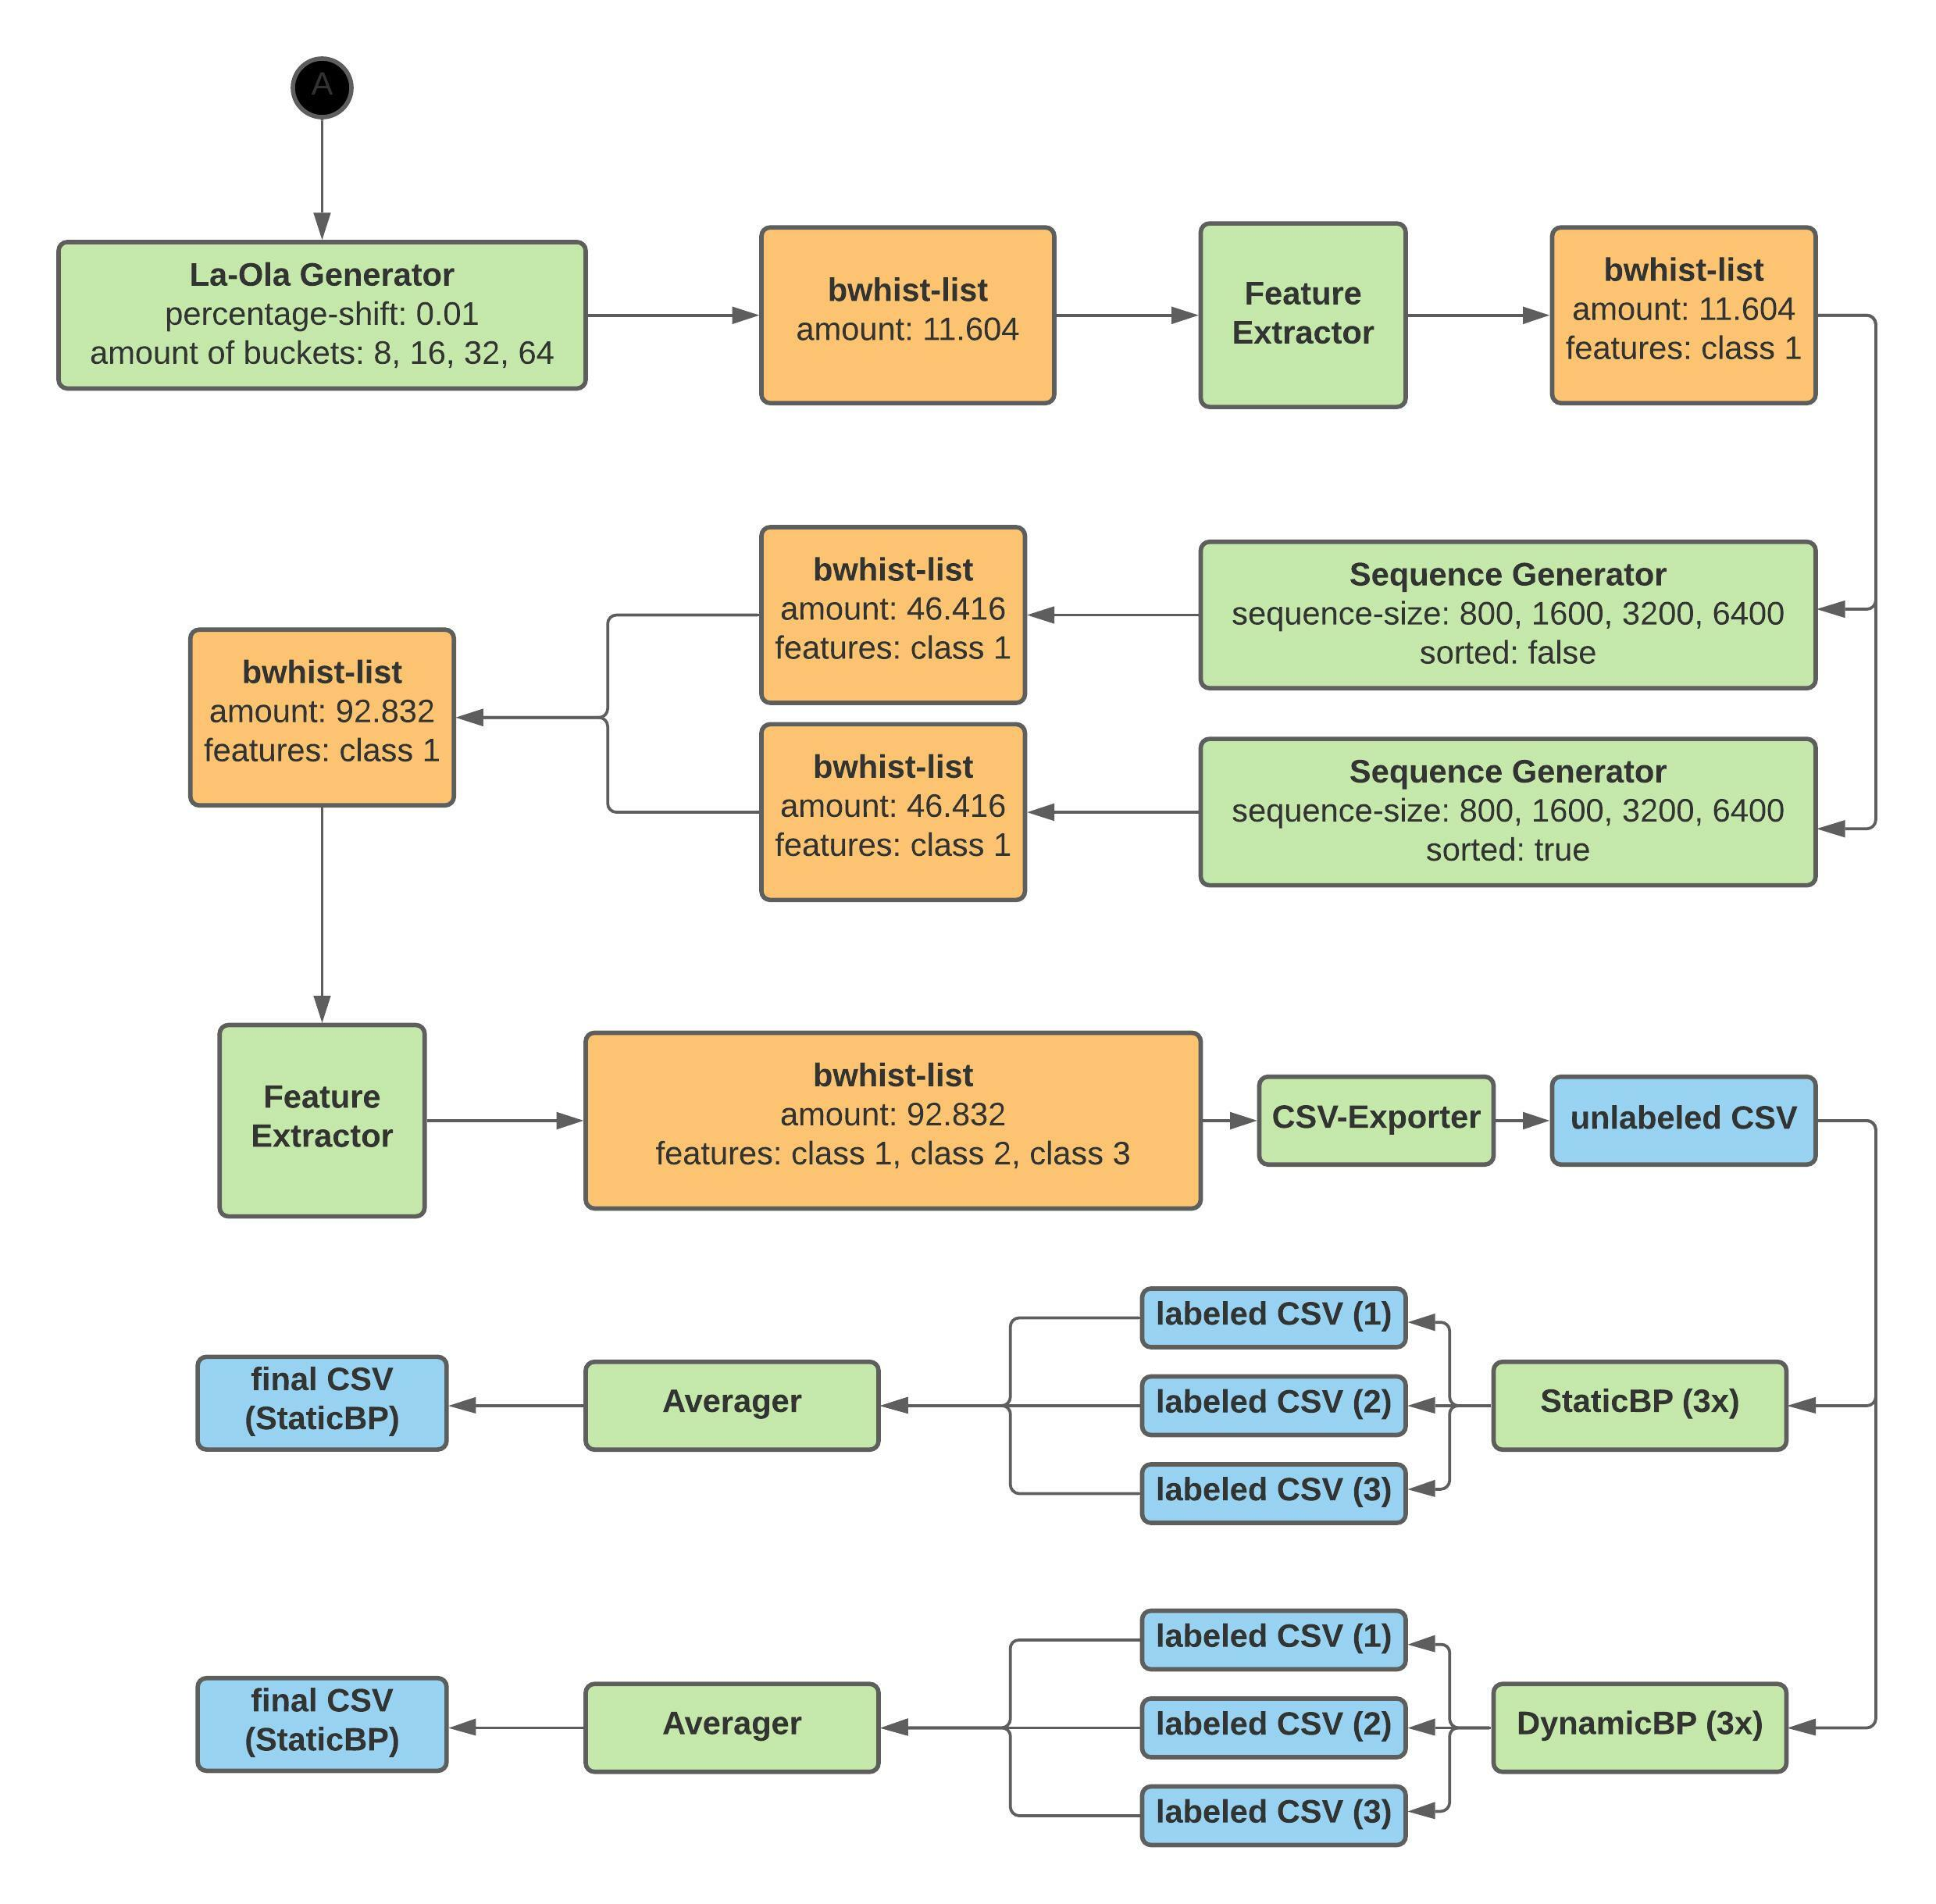
\includegraphics[width = 1.0\textwidth]{pipeline_data_generation}
    \caption{Pipeline for the generation of training data.}
    \label{fig:pipeline-data-generation}
\end{figure}

\section{Validation Pipeline}
After generating the final CSV-File containing the representative data, the ML model can be trained and tuned. The subsequent step is the validation of the ML models against the baseline selection strategy. Figure \ref{fig:pipeline-validation} shows the implementation pipeline for this process. It has to be executed once for each algorithm and for each target value. At first, a fixed subset of 20\% of the entire data set is extracted. The \emph{Algorithm Parameter Sampler} removes the features inputFormat and outputFormat as well as the target values and samples the remaining feature vector for every combination of parameters for the algorithm the data allows, for example the input format can not be smaller than the maximum bitwidth. Hence the sampling process leads to a minimum of 4 feature vectors per data sample if the maximum bitwidth is greater than 32, and a maximum of 16 feature vectors if the maximum bitwidth is smaller than 9. Figure \ref{fig:data-sample} shows an example with 16 possible combinations. 

\begin{figure}[h]
    \centering
    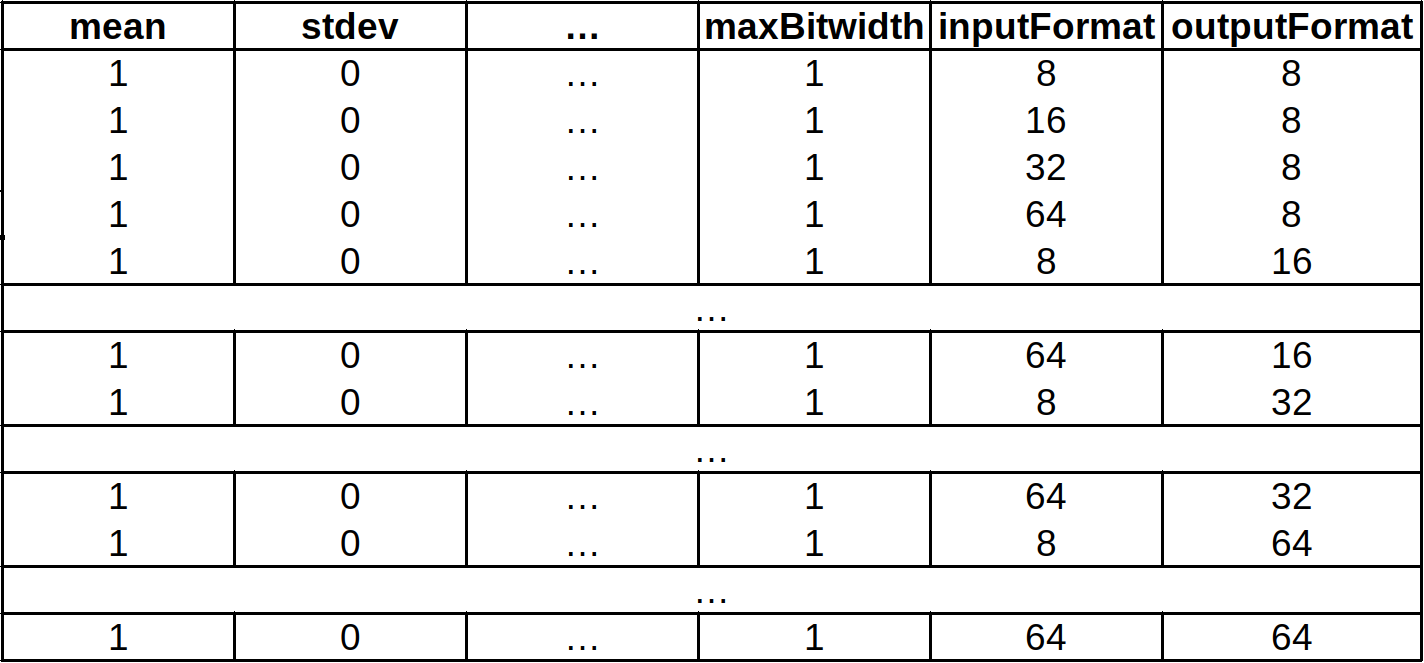
\includegraphics[width = 0.75\textwidth]{data_sample}
    \caption{Example for a feature vector sampled with 16 algorithm parameter combinations.}
    \label{fig:data-sample}
\end{figure}

The next step is the prediction of the target value. Therefore, every feature vector of the sampled test data including the parameterization of the algorithm is passed to the ML model on the one hand and to the baseline on the other hand. This leads to two datasets per algorithm and target value. The first dataset contains the target value predicted by the ML model for each feature vector. The target value of the other one represents the behavior of the baseline strategy which is the selection of the most simple algorithm i.e \emph{StaticBP} with an input format of 64 bit and an output format of 8 bit. This combination of input and output format is the most simple one as it covers all samples while having the best compression rate. 

The CSV-File generated by the data generation pipeline contains a feature vector for every possible algorithm parameter combination. In order to compare the results of the ML model and the baseline, they are passed to the \emph{Accuracy-Slowdown Processor} together with the actual data. The processor determines the minimum of the actual target values over each data sample for all algorithm parameter configuration and the minimum of both the ML model and the baseline. Now it is possible to compare, which algorithm and which parameterization would be chosen by our strategy, which one would be considered the best if the most simple algorithm is used, and which one is actually the best. Given this information, the calculation of the accuracy for the correct algorithm as well as for the correct parameterization is possible. Additionally, the slowdown can be determined, if a wrong parameterization has been chosen.

The same pipeline can be used for the validation against any data set that has been labeled with the algorithm behavior i.e compression rate or compression runtime. For this, the final CSV-File is used in order to train the ML model. This makes sure that training and test data are disjoint. The \emph{Algorithm Parameter Sampler} is then applied directly to the validation data. It is the source for the actual target values that are passed to the \emph{Accuracy-Slowdown Processor}.

\begin{figure}[h]
    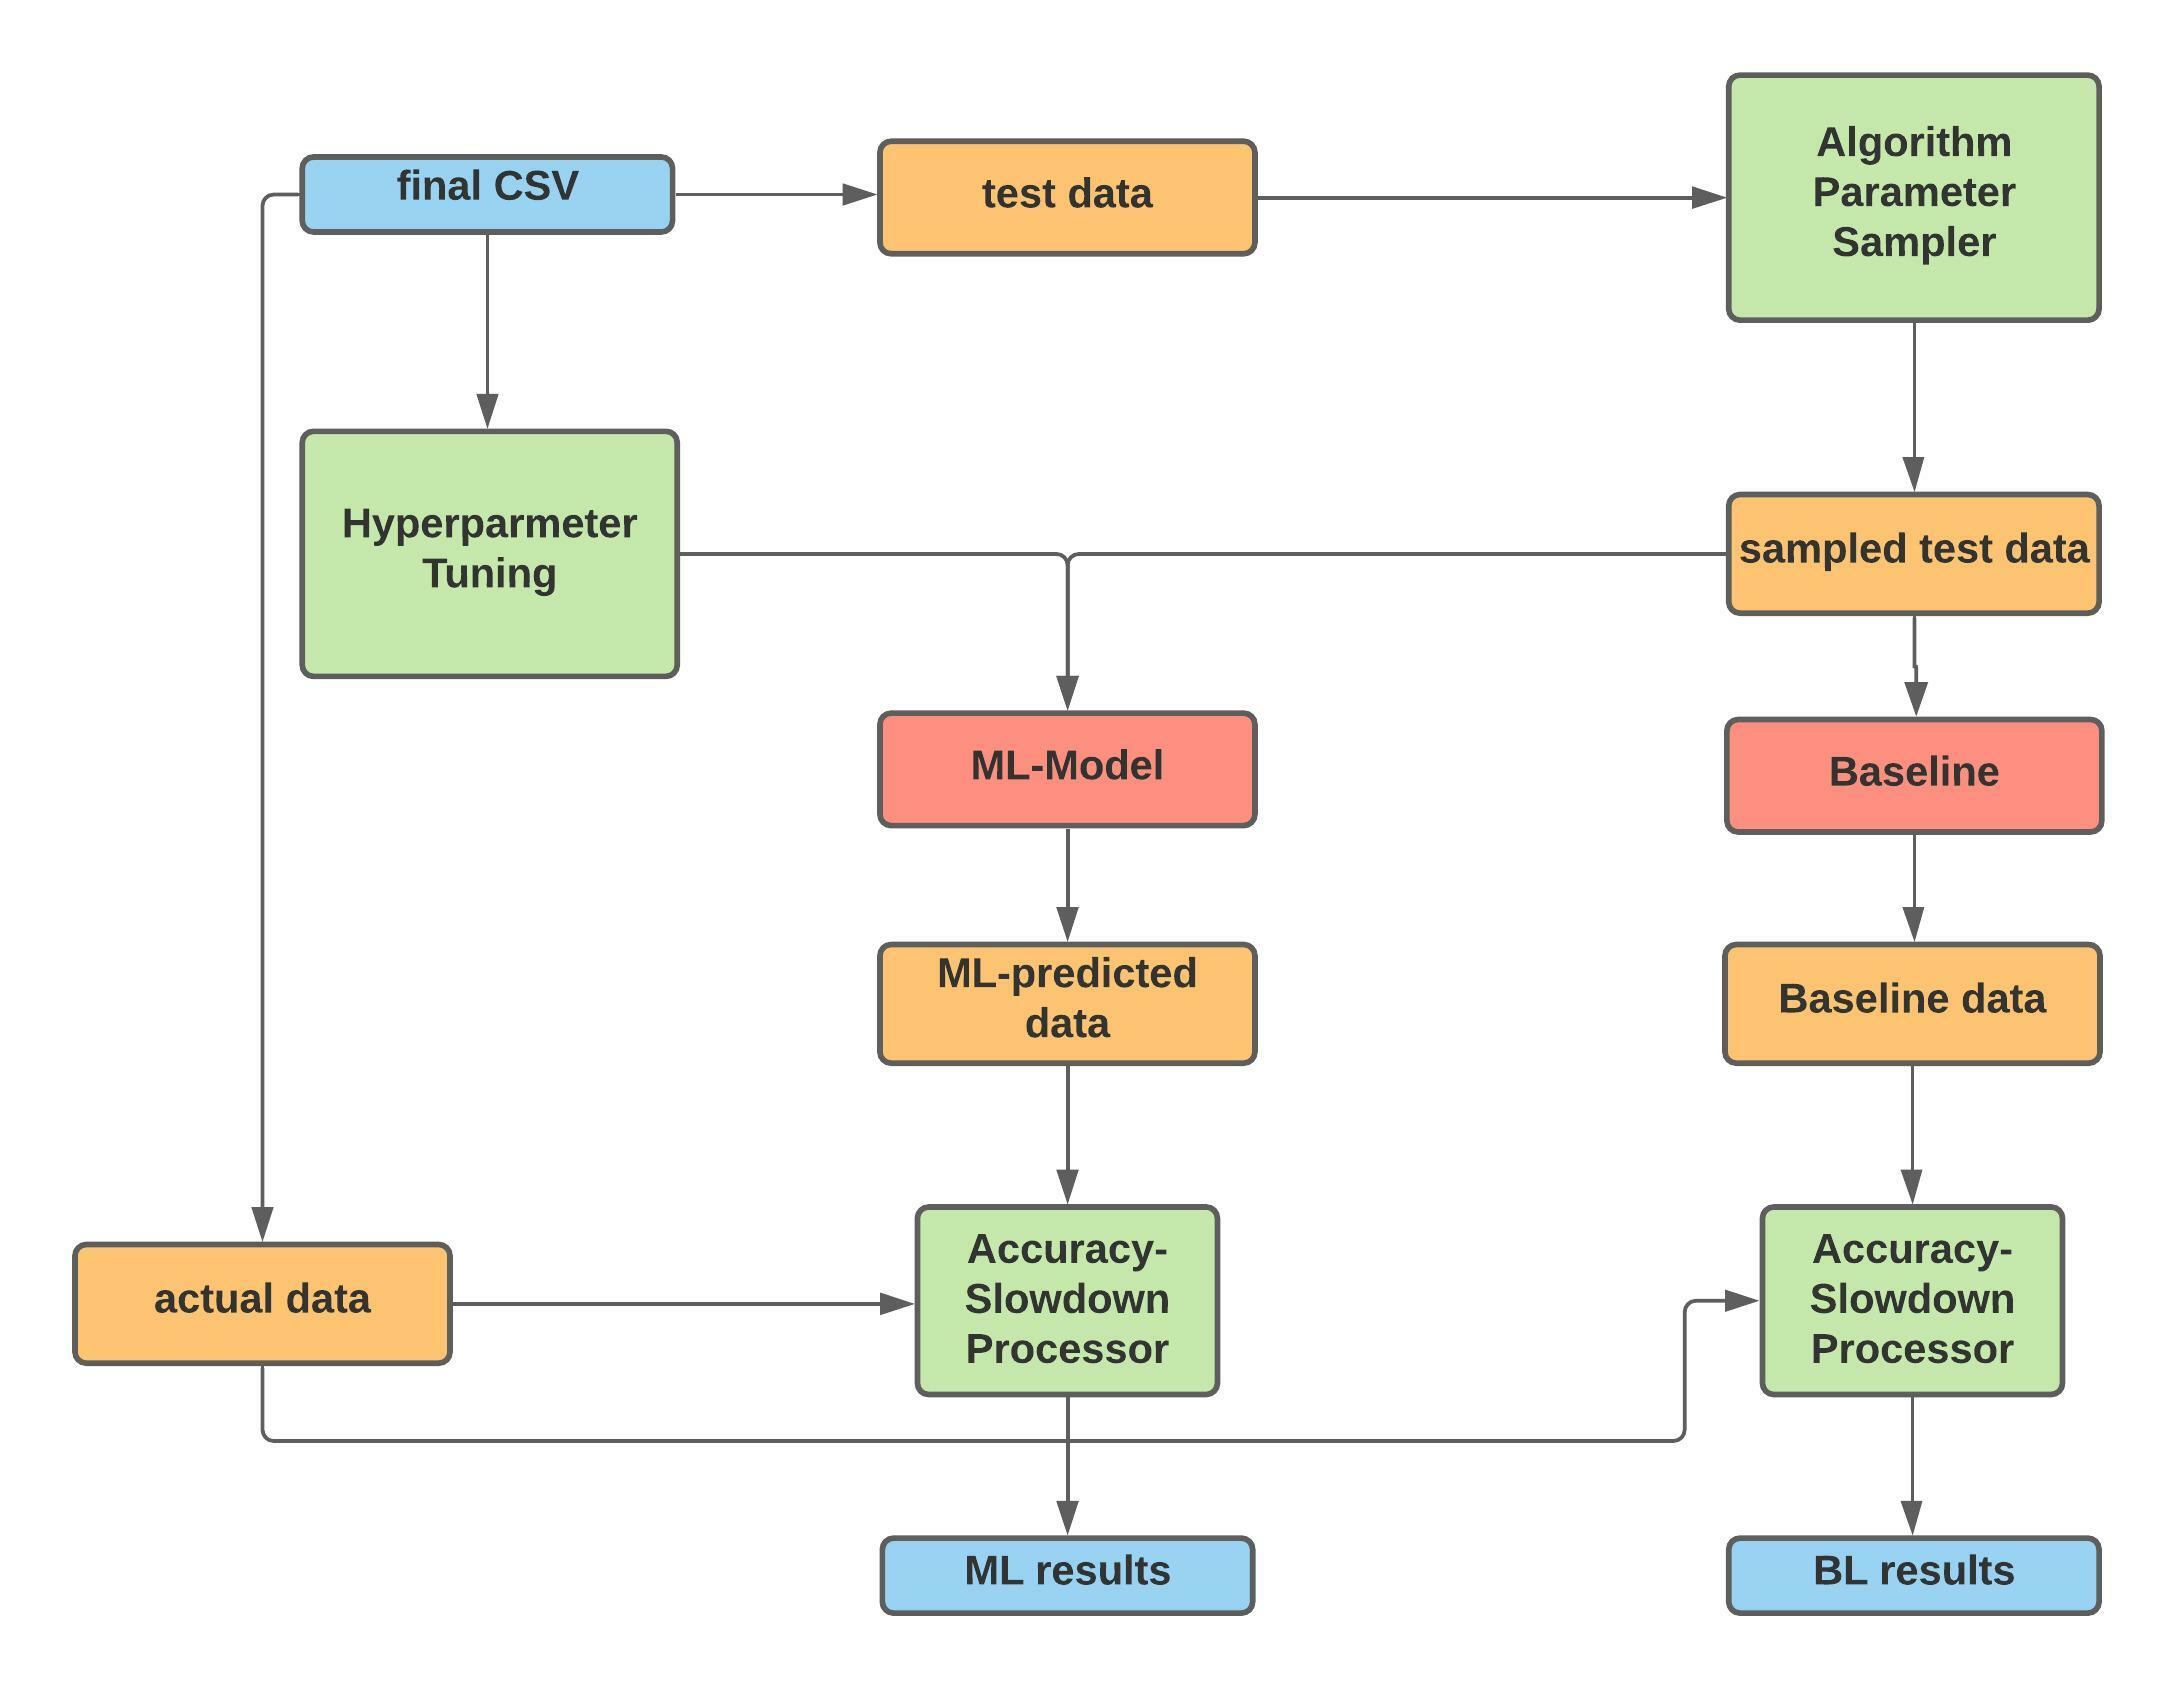
\includegraphics[width = 1.0\textwidth]{validation_pipeline}
    \caption{Pipeline for the validation process of the trained ML-Model.}
    \label{fig:pipeline-validation}
\end{figure}
